
\fullcite{kabe07}

\begin{center}
\fbox{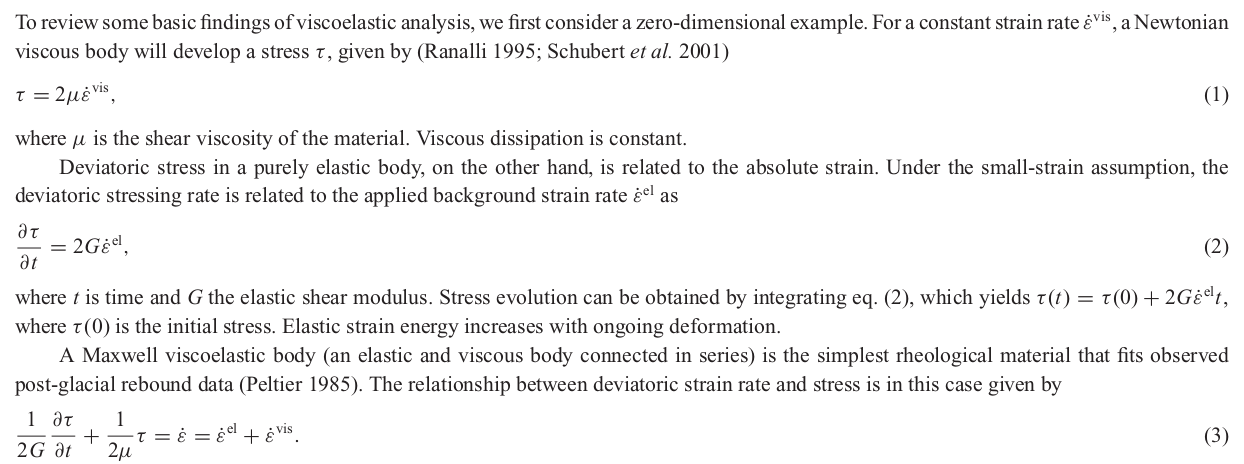
\includegraphics[width=13cm]{images/viscoelasticity/kabe07_a}}
\end{center}
From what follows later we know that ${\bm\tau}$ is the deviatoric stress tensor.
Note the authors talk of a zero-dimensional example here.

\[
{\tau} = 2 \eta \dot{\varepsilon}^{\rm v}
\]
under the small strain assumption:
\[
\frac{\partial { \tau}}{\partial t} = 2 \mu \dot{ \varepsilon}^{\rm e}
\]
\[
\dot{\varepsilon} = \dot{\varepsilon}^{\rm v} + \dot{\varepsilon}^{\rm e}
=
\frac{1}{2\eta} { \tau} + \frac{1}{2\mu} \frac{\partial { \tau}}{\partial t}
\]


\begin{center}
\fbox{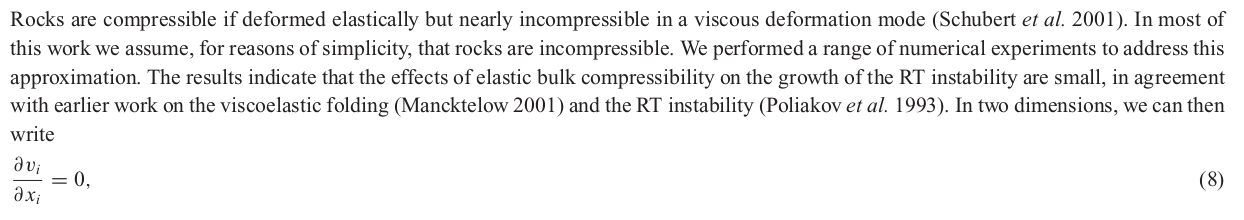
\includegraphics[width=13cm]{images/viscoelasticity/kabe07_b}}
\end{center}

\begin{center}
\fbox{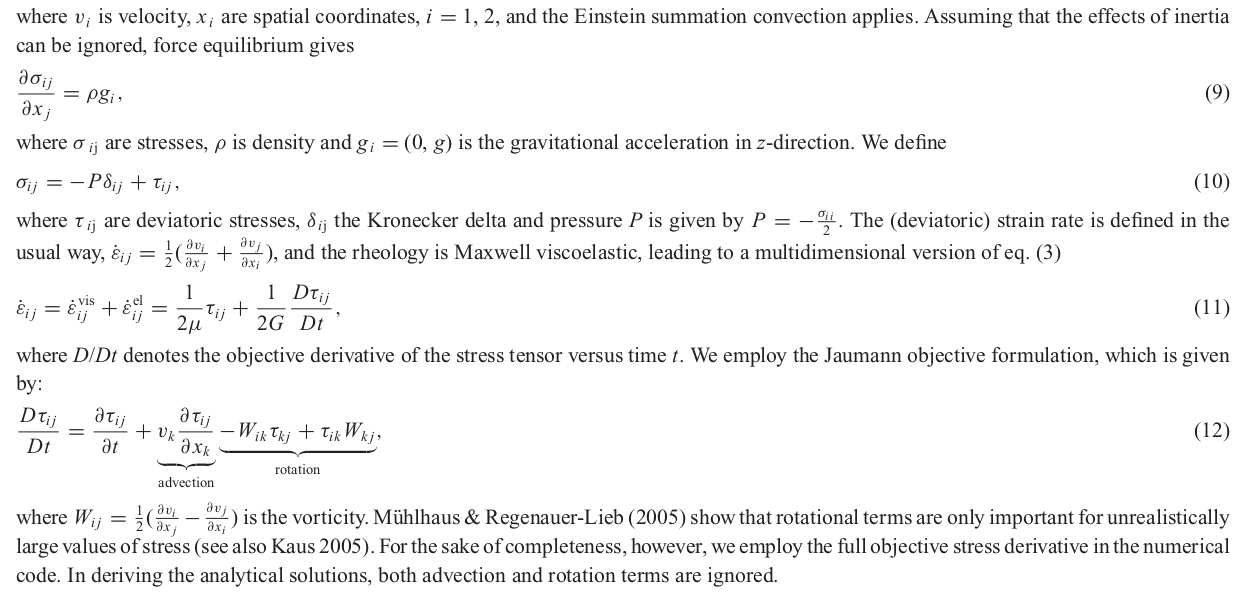
\includegraphics[width=13cm]{images/viscoelasticity/kabe07_c}}
\end{center}

\[
\dot{\bm\varepsilon} = \dot{\bm\varepsilon}^{\rm v} + \dot{\bm\varepsilon}^{\rm e}
=
\frac{1}{2\eta} {\bm \tau} + \frac{1}{2\mu} \frac{{\cal D} {\bm \tau}}{{\cal D} t}
\]
We employ the Jaumann objective formulation, which is given by:
\[
\frac{{\cal D} {\bm \tau}}{{\cal D} t} = \frac{\partial {\bm \tau}}{\partial t}
+ (\vec\upnu \cdot \vec\nabla) {\bm \tau} - \omega \tau + \tau \omega
\]

